%% Produkt 1
%%%%%%%%%%%%%%%%%%%%%%%%%%%%%%
\begin{table}[!htbp] \centering	
	\label{fu:Pir-sensor}
\begin{tabular}{|p{6cm}|p{8cm}|}
	\hline
		\textbf{Løsning}				&HC-SR501, PIR-bevægelsessensor 			\\\hline %Produktnavn
		\textbf{Producent} 			&Vides ikke 			\\\hline 
		\textbf{Tilslutning} 		&- 			\\\hline 
		\textbf{Beskrivelse} 		&En PIR-sensor, når bevægelse er registeret gives et højt eller lavt output(High 3.3 V /Low 0V), alt efter hvad jumperen er indstillet til 			\\\hline 
		\textbf{Krav} 				&Indgående kendskab til PSoC creator 			\\\hline 
		\textbf{Fordele}				&Denne PIR-sensor kræver ingen ekstra HW. Justerbar følsomhed og forsinkelse via potentiometer 			\\\hline 
		\textbf{Ulemper} 			&- 			\\\hline 
		\textbf{Pris} 				&Hentet fra værkstedet på IHA			\\\hline
		\textbf{Link} 				&\url{http://goo.gl/c6GyTL}			\\\hline	
	
		\multicolumn{2}{|c|}
		{									%% Ændre filnavn uden endelse
		\raisebox{-0.91\height}{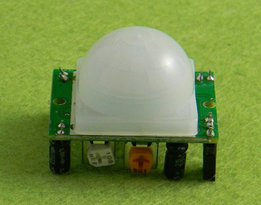
\includegraphics[height=3cm]{filer/forundersoegelse/billeder/Pir_sensor}} 
		} \\\hline	

\end{tabular}
\end{table}
%%%%%%%%%%%%%%%%%%%%%%%%%%%%%%

